\documentclass[12pt, a4paper]{article}
\usepackage[a4paper, top=2cm, bottom=3cm, left=2cm, right=2cm]{geometry}
\usepackage[export]{adjustbox}
\usepackage{graphicx}
\usepackage{mathtools}
\usepackage{hyperref}
\usepackage{amsmath}
\usepackage{amsfonts}
\usepackage{amssymb}
\usepackage[version=4]{mhchem}
\usepackage{stmaryrd}
\usepackage{polyglossia}
\usepackage{fontspec}
\usepackage{ucharclasses}
\usepackage{fancyhdr}
\usepackage{wrapfig}
\usepackage{subcaption}
\usepackage{relsize}
\usepackage{framed}
\usepackage{changepage}
\usepackage{tabularray}
\usepackage{etoolbox}
\usepackage{xstring}
\usepackage{pstricks-add}
\usepackage{tikz}
\usepackage{empheq}
\usepackage{tcolorbox}
\usepackage[european,s traightvoltages, americanresistor, americaninductors]{circuitikz}
\usepackage{pgfplots}
\usepackage{tikz-3dplot}

\usetikzlibrary{
	angles,
	arrows.meta,
	positioning,
	arrows,
	backgrounds,
	calc,
	decorations,
	decorations.markings,
	decorations.pathmorphing,
	fit,
	shapes.arrows,
	shapes.callouts,
	shapes.geometric,
	shapes.misc,
	snakes,
	quotes
}
\pgfplotsset{compat=1.18}
\hypersetup{colorlinks=true, linkcolor=blue, filecolor=magenta, urlcolor=cyan,}
\urlstyle{same}

\setmainlanguage{english}
\setotherlanguages{norwegian, arabic}
\newfontfamily\arabicfont{Noto Naskh Arabic}
% \newfontfamily\lgcfont{CMU Serif}

%%%%%%%%%% Fancy header %%%%%%%%%
\pagestyle{fancy}
\fancyhead[C]{}
\fancyfoot[C]{\medskip\thepage}
\renewcommand{\footrulewidth}{.4pt}
\renewcommand{\headrulewidth}{0pt}

\setlength{\headheight}{14.49998pt}
\addtolength{\topmargin}{-2.49998pt}

\newcommand{\figwidth}{8cm}
\newcommand{\floatfigwidth}{5cm}


%%%%%%%%%% Formatters & Layout %%%%%%%%%
\newcommand{\uprimary}[1]{
	\section*{\center \Huge \underline{#1}}
	\addcontentsline{toc}{section}{\protect\numberline{}#1}
}
\newcommand{\usecondary}[1]{
	\section*{\center \LARGE \underline{#1}}
	\addcontentsline{toc}{section}{\protect\numberline{}#1}
}
\newcommand{\usection}[1]{
	\section*{\LARGE #1}
	\addcontentsline{toc}{subsection}{\protect\numberline{}#1}
}
\newcommand{\usubsection}[1]{
	\section*{\Large #1}
	\addcontentsline{toc}{subsection}{\protect\numberline{}#1}
}
\newcommand{\ussubsection}[1]{
	\section*{\large #1}
	\addcontentsline{toc}{subsection}{\protect\numberline{}#1}
}
\newcommand{\ans}{\bigskip\underline{\textbf{Answer}}}
\newcommand{\ques}[1]{\noparindent\textbf{#1}\doparindent}
\newcommand{\rfloatingimg}[1]{
	\begin{wrapfigure}{r}{\floatfigwidth}
		\includegraphics[max width=\floatfigwidth]{#1}
	\end{wrapfigure}
}
\newcommand{\indentbox}[2]{
	\begin{adjustwidth}{#1}{0pt}
		#2
	\end{adjustwidth}
}
\newcommand{\qa}[3]{
	\noparindent
	\textbf{#1 #2}
	\indentbox{.76cm}{
		\ans
		#3
	}
	\vspace{.75cm}
}
\newcommand{\noskipqa}[2]{
	\noparindent
	\textbf{#1}
	\indentbox{.76cm}{
		\ans
		#2
	}
}
\newcommand{\eqnleft}[1]{
	\begin{flalign*}
		 & #1 &  &
	\end{flalign*}
}
\newcommand{\fullwidthimg}[1]{
	\begin{center}
		\includegraphics[max width=\textwidth]{#1}
	\end{center}
}
\newcommand{\uheading}[2]{
	\uprimary{Module - #1}
	\vspace{-.7cm}
	\usecondary{#2}
}

\newcommand{\note}[1]{
	\begin{tcolorbox}[colframe=green!40!black, colback=green!5!white, title={\textbf{Note}}]
	#1
	\end{tcolorbox}
}


%%%%%%%%%% general constants/symbols %%%%%%%%%
\newcommand\longUparrow{\mathrel{\scalebox{1}[2]{$\uparrow$}}}
\DeclareRobustCommand{\rchi}{{\mathpalette\irchi\relax}}
\newcommand{\irchi}[2]{\raisebox{\depth}{$#1\chi$}}
\newcommand{\term}[1]{\underline{\textbf{#1}}}
\newcommand{\amstr}{\mathring{\textrm{A}}}
\newcommand{\h}{6.626 \times 10^{-34}}
\newcommand{\kB}{1.38 \times 10^{-23}}
\newcommand{\lc}{3 \times 10^{8}}
\newcommand{\uunit}[1]{\mathrm{~#1}}

%%%%%%%%%% Format constants %%%%%%%%%
\newcommand{\doparindent}{\setlength\parindent{.5cm}}
\newcommand{\noparindent}{\setlength\parindent{0pt}}
\graphicspath{ {../images/} }
\NewDocumentCommand{\multiskip}{m}{%
	\begingroup
	\newcount\i  % Define a new counter \i
	\i=0         % Initialize the counter
	\loop
	\ifnum\i<#1
	\bigskip  % Add \bigskip
	\advance\i by 1  % Increment the counter
	\repeat
	\endgroup
}

\newcommand{\termlist}[1]{
	\begin{tcolorbox}[colback=blue!10!white, colframe=blue!50!black, title={Some terms}]
		#1
	\end{tcolorbox}
}


%%%%% dev fx
% startx, starty, endx, endy
\newcommand{\dottedgrid}[4]{
	\draw[thin, dotted] (#1, #2) grid (#3,#4);
	\foreach \i in {#1,...,#3} \node at (\i,-2ex) {\i};
	\foreach \i in {#2,...,#4} \node at (-2ex,\i) {\i};
}
\newcommand{\smallmidarrow}[2]{\tikz \draw[arrows = {-Straight Barb[scale=.8]}, line width=#1] (0,0) -- +(#2,0);}
\newcommand{\midarrow}[2]{\tikz \draw[arrows = {-Straight Barb[scale=1.1]}, line width=#1] (0,0) -- +(#2,0);}

\DefTblrTemplate{caption-tag}{default}{}
\DefTblrTemplate{caption-sep}{default}{}
\DefTblrTemplate{caption-text}{default}{}
\DefTblrTemplate{contfoot-text}{default}{}
\DefTblrTemplate{conthead-text}{default}{}

\usepackage{tikz}
\usepackage{listofitems}
\usepackage{xargs}
\usepackage{fp}
\usetikzlibrary{3d,calc,patterns,quotes,angles,perspective}

\newcommandx{\shadedPlane}[6][5=blue, 6=0.8]{
	\readlist\a{#1}%
	\readlist\b{#2}%
	\readlist\c{#3}%
	\readlist\d{#4}%
	\coordinate (P1) at (\a[1], \a[2], \a[3]);
	\coordinate (P2) at (\b[1], \b[2], \b[3]);
	\coordinate (P3) at (\c[1], \c[2], \c[3]);
	\coordinate (P4) at (\d[1], \d[2], \d[3]);
	\fill[pattern=north east lines, pattern color=#5, opacity=#6]
	(P1) -- (P2) -- (P3) -- (P4)-- cycle;
	\draw[thick, color=#5, opacity=#6]
	(P1) -- (P2) -- (P3) -- (P4) -- cycle;
}

\newcommandx{\axes}[2][1=1, 2=1.3]{
	\FPeval\axside{#1 * #2}
	\draw[->, red] (0,0,0) -- (\axside,0,0) node[anchor=north east] {$x$};
	\draw[->, green] (0,0,0) -- (0,\axside,0) node[anchor=north west] {$y$};
	\draw[->, blue] (0,0,0) -- (0,0,\axside) node[anchor=south] {$z$};
}
\newcommandx{\wirecube}[2][2=1pt]{
	% vertices of the cube & plane
	\coordinate (A) at (0,0,0);
	\coordinate (B) at (#1,0,0);
	\coordinate (C) at (#1,#1,0);
	\coordinate (D) at (0,#1,0);
	\coordinate (E) at (0,0,#1);
	\coordinate (F) at (#1,0,#1);
	\coordinate (G) at (#1,#1,#1);
	\coordinate (H) at (0,#1,#1);

	% Draw the edges of the cube
	\draw[thick] (A) -- (B) -- (C) -- (D) -- cycle;
	\draw[thick] (E) -- (F) -- (G) -- (H) -- cycle;
	\draw[thick] (A) -- (E);
	\draw[thick] (B) -- (F);
	\draw[thick] (C) -- (G);
	\draw[thick] (D) -- (H);

	% Add points to illustrate vertices
	\foreach \i in {(A), (B), (C), (D), (E), (F), (G), (H)} {
			\filldraw[black] \i circle (#2);
		}
}

\newcommand{\wirecubewithlabels}[2]{
	\wirecube{#1}[#2]

	% Label the side lengths

	\coordinate (A) at (0,0,0);
	\coordinate (B) at (#1,0,0);
	\coordinate (D) at (0,#1,0);
	\coordinate (E) at (0,0,#1);

	\node at ($(A)!0.8!(B)$) [above] {$\vec{a}$};
	\node at ($(A)!0.7!(D)$) [above right] {$\vec{b}$};
	\node at ($(A)!0.7!(E)$) [above] {$\vec{c}$};
	\draw[thick, ->] (A) -- (B);
	\draw[thick, ->] (A) -- (D);
	\draw[thick, ->] (A) -- (E);
	\pic [blue,draw,angle radius=0.25cm] {angle=B--A--E};
	\pic [green,draw,angle radius=0.25cm] {angle=D--A--B};
	\pic [red,draw,angle radius=0.25cm] {angle=D--A--E};

	\node[color=blue, scale=.8] at (.4,0.4,0) {$\gamma$};
	\node[color=green, scale=.8] at (.7,0,.7) {$\beta$};
	\node[color=red, scale=.8] at (-0.3,0.3,0.3) {$\alpha$};
}

\newcommand{\smallmidarrow}[2]{\tikz \draw[arrows = {-Straight Barb[scale=.8]}, line width=#1] (0,0) -- +(#2,0);}
\newcommand{\midarrow}[2]{\tikz \draw[arrows = {-Straight Barb[scale=1.1]}, line width=#1] (0,0) -- +(#2,0);}
\newcommand{\millerDiagramQuad}[6]{
	\begin{tikzpicture}[
			scale=#6,
			x={(-.45cm, -.4cm)},
			y={(1cm, 0cm)},
			z={(0cm, 1cm)}
		]
		\axes[#5]
		\shadedPlane{#1}{#2}{#3}{#4}

		\wirecube{#5}[0pt]

	\end{tikzpicture}
}

\newcommand{\millerDiagram}[5]{
	\millerDiagramQuad{#1}{#2}{#3}{#3}{#4}{#5}
}

\newcommand{\doubleCylinder}[3]{
	\draw (0,0) ellipse (#1 and #1*2);
	\draw (0,#1*2) -- ++(#3, 0);
	\draw (0,-#1*2) -- ++(#3, 0);

	\draw (0,0) ellipse (#2 and #2*2);
	\draw (0,#2*2) -- ++(#3, 0);
	\draw (0,-#2*2) -- ++(#3, 0);
}

% x,y, r, y-scalar, x-length, y-shear, color
\newcommand{\cylinder}[7]{
	\begin{scope}[shift={(#1, #2)}]
		\draw[fill=#7, draw=black] (#5, #4*#3+#6) arc (90:-80:#3 and #4*#3) -- ++(-#5, -#6) arc (-80:90:#3 and #4*#3) -- cycle;
		\draw[fill=#7, draw=black] (0, 0) ellipse (#3 and #4*#3);
	\end{scope}
}

\begin{document}
\section*{Integral Calculus}
\begin{enumerate}
  \item $\int \ln (x) d x$
\end{enumerate}

$=\int \ln (x) \times 1 d x=\ln (x) \int 1 d x--\int \frac{1}{x} \cdot \int 1 d x d x \quad \int u 0=u \int v-\int a \int f$

$$
\begin{aligned}
& =x \ln (x)-x+c \\
& =(x-1) \ln (x)+c
\end{aligned}
$$

\begin{enumerate}
  \setcounter{enumi}{1}
  \item $\int e^{x} x^{5} d x=\int x^{5} e^{x} d x=x^{5} \int e^{x}-\underbrace{\int 5 x^{4} \cdot \int^{x} d x}_{-x_{1}}$
\end{enumerate}

$$
\begin{aligned}
& =x^{5} e^{x}-5 \int x^{4} e^{x} \\
& =x^{5} e^{x}-5 x^{4} e^{x}+20 x^{3} e^{x}-60 x^{3} e^{x}+120 x e^{x} \\
& =x^{5} e^{x}-5 x^{4} e^{x}+20 x^{3} e^{x}-60 x^{2} e^{x}+120 x e^{x}-120 e^{x}
\end{aligned}
$$

$3 \int\left(x^{5}+8 x^{2}+1\right) d x=\frac{x^{6}}{6}+\frac{8}{3} x^{3}+x+c$

\begin{enumerate}
  \setcounter{enumi}{4}
  \item $\int \frac{2(x+5)}{x^{2}+10 x+25} d \frac{2}{x+5}=2 \ln (x+5)+c$
\end{enumerate}

5). $\int \sin (3 x) \cdot e^{2 x} d x \sim\left\{\int e^{a x} \cdot \sin (b x) d x=\left[\frac{e^{a x}}{a^{2}+b^{2}}[a \sin (b x)-b \cos (b x)]\right\}\right.$ $\sim \frac{e^{2 x}(2 \sin (3 x)-3 \cos (3 x)]}{13}\left\{\int e^{a x \cos }(b x) d x=\frac{e^{a x}}{a^{2}+b^{2}}[a \cos (b x)+b \sin (b x)]\right\}$ 6. $\int e^{x}(\sec (x)+\sec (x) \operatorname{ton}(x)) d x$ $8 \int x^{2} \cdot \tan ^{-1}(x)$

$$
\begin{aligned}
& =\int \tan ^{-1}(x) x^{2}-d x \\
& =\tan ^{-1}(x) \cdot \frac{x^{3}}{3}-\int \frac{1}{1+x^{2}} \cdot \frac{x^{3}}{3} d x \quad \begin{array}{ll}
x^{3} \rightarrow t \\
& d t=3 x^{2} \cdot d x
\end{array} \\
& \int \frac{x}{1+x^{2}} \cdot x^{2} d x \\
& \Rightarrow \quad \frac{1}{2} \int \frac{t-1}{z} d t \Rightarrow \frac{1}{2} \int 1-\frac{1}{2} \int \frac{1}{t} \\
& =\frac{1}{2}\left(x^{2}+1\right)-\frac{1}{2} \ln \left(x^{2}+1\right) \\
& \Rightarrow \tan ^{-1}(x) \cdot \frac{x^{3}}{3}-\frac{1}{6}\left(x^{2}+1\right)+\frac{1}{6} \ln \left(x^{2}+1\right)+c \\
& \int \frac{x+1}{x^{2}+6 x+25}= \\
& \rightarrow \frac{1}{2} \int \frac{2 x+6}{x^{2}+6 x+25} d x-2 \int \frac{d x}{x^{2}+6 x+25} \quad \begin{array}{ll}
2 x+6=a \\
& b=x+1-(2 x+6)
\end{array} \\
& t_{1}=x^{2}+6 x+68
\end{aligned}
$$

\begin{center}
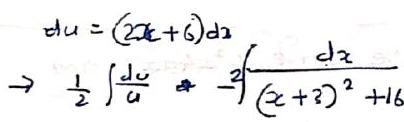
\includegraphics[max width=\textwidth]{2024_07_21_a4d038e3d75ef384087fg-1(1)}
\end{center}

\begin{center}
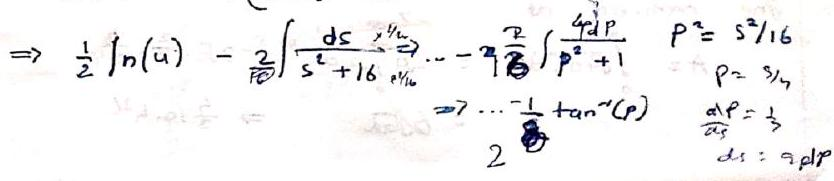
\includegraphics[max width=\textwidth]{2024_07_21_a4d038e3d75ef384087fg-1(2)}
\end{center}

$$
\begin{aligned}
& \begin{array}{l}
\Rightarrow \frac{\ln (4)}{2}-\frac{1}{2} \tan ^{-1}\left(\frac{5}{4}\right) \\
\Rightarrow \frac{\ln \left(x^{2}+6 x+25\right)}{2}-\frac{1}{2} \tan ^{-1}\left(\frac{x+3}{4}\right)
\end{array}
\end{aligned}
$$

Quadrature

wapticolise of area of curve bounded by a Gundary finding

Area bounded by a curve $y=f(x)$ within $[a, b]$ in $x$-axis is

$$
A=\int_{a}^{b} y d x \equiv \int_{a}^{b} f(x) d x
$$

Also if the curve is $x=f(y)$, then area within $[a, b]$ in $y$-ayis is:

$$
A=\int_{a}^{b} x d x y=\int_{a}^{b} f(y) d y
$$

\begin{itemize}
  \item If two curves $y_{1}=f(x) \quad y_{2}=\phi(x)$ intersects at the points whuse coordinates are $(a, .).(b, \ldots)$ then the area enclosed by curve is givenby. $A=\int_{a}^{b}(f(x)-\phi(x)) d x$
\end{itemize}

1 Find area bounded by the curve, $y^{2}=4 a x$ and the ordinatif at $x=h$,\\
A) $\quad A=\int_{0}^{h} \sqrt{4 a x} d x \left\lvert\,=2 \sqrt{a} \sqrt{x} d x=2 \sqrt{a} \cdot \frac{2}{3} \cdot \frac{b}{x^{3 / 2}}\right.$

$$
\text { a }=6 \sqrt{6 o h} \quad \Rightarrow \frac{4}{3} \sqrt{a} \cdot h^{3 / 2}
$$

2 Find area erelused by curve $\frac{x^{2}}{a^{2}}+\frac{y^{2}}{b^{2}}=1$

A.)

$$
\begin{aligned}
& \text { let } y=0, \quad \therefore x=4 \\
& x=a, \quad \therefore y=b
\end{aligned}
$$

\begin{center}
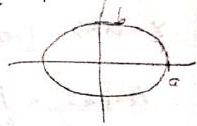
\includegraphics[max width=\textwidth]{2024_07_21_a4d038e3d75ef384087fg-1}
\end{center}

\section*{$\therefore c$ }
$\therefore y=b \sqrt{1-\frac{x^{2}}{a^{2}}}=\frac{a b}{a} \sqrt{a^{2}-x^{2}}$

$\therefore A=4 \int_{0}^{a} y d x=4 \frac{a b}{a} \int_{0}^{a} \sqrt{a^{2}-x^{2}} d x$

$=4 \frac{a b}{a}\left[\frac{x}{2} \sqrt{a^{2}-x^{2}}-\frac{a^{2}}{2} \sin ^{-1}\left(\frac{x}{a}\right)\right]_{0}^{c}$

$=4 \frac{a b}{a} \cdot \frac{a^{2}}{2} \sin ^{-1}(1)$

$=\pi a b$

\begin{enumerate}
  \setcounter{enumi}{2}
  \item Find area enclused blw lineff and curve $y=x^{2}-6 x+4$\\
A) $y=1-2 x=\left\{x^{2}-6 x+4 \Rightarrow x^{2}-4 x+3=0\right.$
\end{enumerate}

$f=x^{2}-6 x+4, \phi=1-2 x$

$=044 \rightarrow 0 \pm 1 \Rightarrow 13$

$\therefore$ Area $=\int_{10}^{3}((f-\phi) d x$

10/1 4find area bounded by the curve $y=3 x-x^{2}$ the $x$-axis and line $x=3, x=0$

A) Area $=\int_{0}^{3}\left(3 x-x^{2}\right) d x$

$$
\left.=\frac{3}{2} x^{2}-\frac{x^{3}}{3}\right]_{0}^{3}=\frac{27}{2}-9=\frac{9}{2}
$$

\begin{enumerate}
  \setcounter{enumi}{4}
  \item Find ane of asteroid: $x^{2 / 3}+y^{2 / 3}=a^{2 / 3}$
\end{enumerate}

A) $x^{2 / 2}+y^{2 / 3}=a^{2 / 3}$

$$
y=\left(a^{2 / 3}-x^{2 / 3}\right)^{3 / 2}
$$

$\therefore$ Area of asteroid $=4 \int_{0}^{a}\left(a^{2 / 3}-x^{2 / 2}\right)^{3 / 2} d x=: A$

\begin{center}
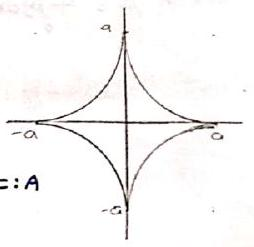
\includegraphics[max width=\textwidth]{2024_07_21_a4d038e3d75ef384087fg-2(3)}
\end{center}

$$
\begin{aligned}
& a \sin ^{3}(\theta)=0 \Rightarrow \theta=0 \\
& \therefore d x=3 a \sin ^{2}(\theta) \cos (\theta) d \theta \\
& a \sin ^{3}(\theta)=a \Rightarrow \theta=\pi / 2 \\
& \left.\therefore A \equiv 4 \int_{0}^{\pi / 2}\left(a^{2 / s}-a^{2 / 3} \sin ^{2}(\theta)\right)^{3 / 2}\right) 3 a \sin ^{2}(\theta) \cos (\theta) d \theta \\
& =4 \int_{0}^{\pi / 2} a\left(1-\sin ^{2}(\theta)\right)^{2 / 2} \cdot 3 a \sin ^{2}(\theta) \cos (\theta) d \theta \\
& =012 a^{2} \int_{0}^{\pi / 2} \cos ^{3}(\theta) \sin ^{2}(\theta) \cos (\theta) d \theta \\
& =12 a^{2} \int_{0}^{\pi / 2} \cos ^{4}(\theta) \sin ^{2}(\theta) d \theta \\
& =12 a^{2} \cdot \frac{3 \times 1 \times 1}{6 \times 4 \times 2} \times \frac{\pi}{2}
\end{aligned}
$$

\begin{center}
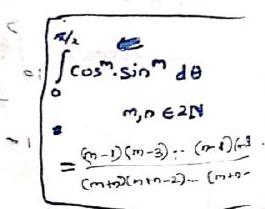
\includegraphics[max width=\textwidth]{2024_07_21_a4d038e3d75ef384087fg-2}
\end{center}

$$
\begin{aligned}
& =\frac{3}{8} a^{2} \pi \\
& \text { fund } m, n \in 2^{r+1}
\end{aligned}
$$

Length (perimeter) of Carve (Rectification)

\begin{itemize}
  \item let $y=f(x)$. length of carve from $[0, a]$
\end{itemize}

$$
d=\int_{0}^{\infty} d x \sqrt{1+\left(\frac{d y}{d x}\right)^{2}} d x
$$

If $x=f(y)$

$$
L=\int_{0}^{a} \sqrt{1+\left(\frac{d x}{d y}\right)^{2}} d y
$$

\begin{center}
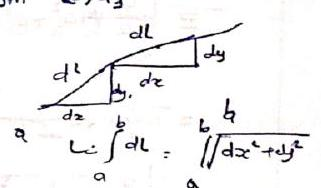
\includegraphics[max width=\textwidth]{2024_07_21_a4d038e3d75ef384087fg-2(2)}
\end{center}

\begin{itemize}
  \item If $x=f(t), y=\phi(t), L=\int_{0}^{a} \sqrt{\left(\frac{d x}{d b}\right)^{2}+\left(\frac{d y}{d b}\right)^{2}} \cdot d t$
  \item If $\gamma^{\prime}=f(\theta), \quad L=\int_{0}^{a} \sqrt{\gamma^{2}+\left(\frac{d \gamma}{d \theta}\right)^{2}} \cdot d \theta$
\end{itemize}

\begin{center}
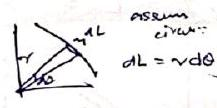
\includegraphics[max width=\textwidth]{2024_07_21_a4d038e3d75ef384087fg-2(1)}
\end{center}

\begin{enumerate}
  \item Find the length of the carve $y^{2}=4 a x$, measure from the vertex to one extremity of Lotus rectum
\end{enumerate}

$\dot{A} \quad L=\int_{0}^{a} \sqrt{1+\left(\frac{d y}{d x}\right)^{2}} d x$.

$$
\text { - } \begin{aligned}
y & =2 \sqrt{a x} \\
\frac{d y}{d x} & =\frac{a}{\sqrt{a x}}=\sqrt{\frac{a}{x}} \\
\therefore L & =\int_{0}^{a} \sqrt{1+\frac{a}{x}} d x \\
& =\int_{0}^{a} \frac{\sqrt{x+a}}{\sqrt{x}} d x
\end{aligned}
$$

$$
\text { 2. } \frac{1}{2} \frac{5}{\sqrt{\operatorname{an}}}
$$

\begin{center}
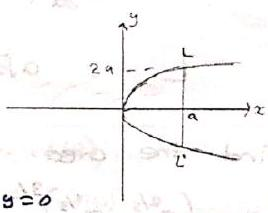
\includegraphics[max width=\textwidth]{2024_07_21_a4d038e3d75ef384087fg-2(4)}
\end{center}

$$
\begin{aligned}
& x=0, y=0 \\
& x=a, y=2 a \\
& x=\frac{y^{2}}{4 a} \quad \frac{d x}{d y}=\frac{y}{2 a} \\
& L=\int_{0}^{2 a} \sqrt{1+\frac{y^{2}}{4 a^{2}}} d y \\
& =\frac{1}{2 a} \cdot \int_{0}^{2 a} \sqrt{(2 a)^{2}+y^{2}} d y
\end{aligned}
$$

$$
\begin{aligned}
& \sinh ^{-1}(x)=\ln \left(x+\sqrt{x^{2}+a^{2}}\right) \\
& \therefore=\left[\frac{1}{2} \sqrt{4 a^{2}+y^{2}}+\frac{\left(2 \partial^{2}\right.}{2} \ln \left(y+\sqrt{4 a^{2}+y^{2}}\right)\right]_{0}^{2 a} \\
& =\frac{1}{2 a} \cdot\left(2 a^{2} \sqrt{2}+\frac{2 a^{2}}{2 a}(2 a+2 a \sqrt{2})\right) \\
& L=a \sqrt{2}+\ln (2 a(1+\sqrt{2})) \\
& L=\frac{1}{2 a}\left[\frac{y}{2} \sqrt{y^{2}+a^{2}}+\frac{2 a^{2}}{2} \sinh h^{-1}\left(\frac{y}{a}\right)\right]_{0}^{24}
\end{aligned}
$$


\begin{align*}
& =\frac{1}{2 a}\left(\frac{2 a}{2} \sqrt{(2 a)^{2}+(2 a)^{2}}+\frac{2 a^{2}}{2} \sinh ^{-1}\left(\frac{2 a}{2 a}\right)\right) \\
& =\frac{1}{2 a}\left(a^{2} 2 \sqrt{2}+2 a^{2} \ln (1+\sqrt{2})\right)^{\prime} \\
& L=a \sqrt{2}+a \ln (1+\sqrt{2})
\end{align*}


\begin{enumerate}
  \setcounter{enumi}{1}
  \item Find the area of astroid $x^{2 / 3}+y^{2 / 3}=a^{2 / 3}$\\
A) $y=\left(a^{2 / 3}-x^{2 / 3}\right)^{3 / 2}$
\end{enumerate}

$$
\begin{aligned}
\text { Area of single piece } & =\int_{0}^{a} y \cdot d x \\
& =\int_{0}^{a}\left(a^{2 / 3}-x^{2 / 3}\right)^{3 / 2} d x
\end{aligned}
$$

let $x=a \sin ^{3}(\theta) \Rightarrow d x=3 a \sin ^{2}(\theta) \cdot \cos (\theta) \cdot d \theta$

$\rightarrow$ bounds are $x=0 \mapsto \theta=0$

$$
x=a \mapsto \theta=\pi / 2
$$

$\therefore$ Area of single piece $=\int_{0}^{\pi / 2}\left(a^{2 / 3}-0^{2 / 3} \sin ^{2} \theta\right)^{3 / 2} \cdot 3 a \sin ^{2} \theta \cdot \cos (\theta) \cdot d \theta$

$$
\begin{aligned}
& =3 a^{2} \int_{0}^{\pi / 2} \cos ^{4}(\theta) \sin ^{2}(\theta) d \theta \\
& =3 a^{2} \times \frac{3 \times 1 \times 1}{6 \times 4 \times 2} \times \frac{\pi}{2}=\frac{3 \pi}{32} a^{2}
\end{aligned}
$$

$\therefore$ Area of astroid $=4 \times \frac{3 \pi a^{2}}{32}=\frac{3}{8} \pi a^{2}$

$$
\begin{aligned}
\int_{0}^{\pi / 2} \cos ^{m}(\theta) \sin ^{n}(\theta) d \theta= & (m-1)(m-3)(m-5) \cdots(m-\cdots) \\
& \times(n-1)(n-3)(n-5) \cdots \frac{(n-\cdots)}{20} \\
& \times \frac{1}{(m+n)(m+n-2)(m+n-4)(m+n-\cdots)} \frac{\pi}{2}
\end{aligned}
$$

Area of Polar functions

$$
\frac{1}{2} \int_{a}^{b} \tau^{2} d \theta
$$

\begin{enumerate}
  \item Find whole area of circle: $r=2 \operatorname{acos}(\theta)$,
\end{enumerate}

$$
\text { - Cardioid: } r=a(1-\cos (\theta))
$$

A) Circle

$$
\begin{aligned}
& \text { let } r=0 \Rightarrow \theta=\frac{\pi}{2} \\
& r=2 a \Rightarrow \theta=0 \\
& \therefore \text { Area }=2 \int_{0}^{\pi / 2} \frac{1}{2} \cdot r^{2} d \theta=4 a^{2} \int_{0}^{\pi / 2} \cos ^{2}(\theta) d \theta \\
& =4 a^{2} \cdot \frac{1}{2} \pi=\pi a^{2} \\
& \int_{0}^{\pi / 2} \cos ^{2}(\theta) d \theta=\frac{(n-1)(n-s) \ldots(n-\ldots)}{n(n-2)(n-4)(n-\cdots)} \times \frac{\pi}{2}
\end{aligned}
$$

Cardiad

$$
\begin{aligned}
& r=a(1-\cos (\theta)) \\
& r=0 \Rightarrow \theta=\pi \quad, \therefore \theta \in[0, \pi] \\
& \begin{aligned}
& \therefore \text { Area }=2 \int_{0}^{\frac{1}{2}} r^{2} d \theta= a^{2} \int_{0}^{\pi} 4(1-\cos (\theta))^{2} d \theta \\
&= a^{2} \int_{0}^{\pi}\left(2 \sin ^{2} \frac{\theta}{2}\right)^{2} d \theta=4 a^{2} \int_{0}^{\pi} \sin ^{4}(\theta / 2) d \theta \\
& \text { let } \phi=\theta / 2 \Rightarrow \phi \in[0, \pi / 2]
\end{aligned}
\end{aligned}
$$

$\therefore A=4 a^{2} \int_{0}^{\pi / 2} \int \sin ^{2}(\phi) d \phi=8 a^{2} \int_{0}^{\pi / 2} \sin ^{4}(\phi) d \phi$

$$
=8 a^{2} \times \frac{3 \times 1}{4 \times 2} \times \frac{\pi}{2}=\frac{3}{2} \pi c^{2}
$$

\section*{Surface area of "Curves}
\begin{itemize}
  \item Revolving about $x$-axis-: $\int_{a}^{b} 2 \pi y d s$ where $d s=\sqrt{1+\left(\frac{d y}{d x}\right)^{2}} \cdot d x$ in cartesian
\end{itemize}

$$
\begin{aligned}
& d s=\sqrt{\left(\frac{d r}{d t}\right)^{2}+\left(\frac{d y}{d t}\right)^{2}} d t \text { in parametric } \\
& d s=\sqrt{r^{2}+\left(\frac{d d}{d \theta}\right)^{2}} d \theta \text { in polar }
\end{aligned}
$$

\begin{enumerate}
  \item Find avea of the surface generated by revolving the parabola $y^{2}=4 a x$ about $x$ axi from origin to $x=a$ A. $\quad A=\int_{0}^{a} 2 \pi y \cdot d s$
\end{enumerate}

$$
\begin{aligned}
& \frac{d y}{d x}=2 \sqrt{a} \cdot \frac{1}{2} \frac{1}{\sqrt{x}}=\sqrt{\frac{a}{x}} \quad y=2 \sqrt{a x} \\
& \begin{aligned}
\therefore d S=\sqrt{1+\left(\frac{d y}{d x}\right)^{2}} d x & =\sqrt{\frac{x+a}{x}} d x \\
\therefore A=\int_{0}^{a} 2 \pi y \cdot d s & =2 \pi \int_{0}^{a} 2 \sqrt{a x} \sqrt{\frac{x+a}{x}} d x \\
& =4 \pi \sqrt{a} \int_{0}^{a} \sqrt{x+a} d x \\
& =\frac{8}{3} \pi \sqrt{a}\left[(x+a)^{3 / 2}\right]_{0}^{a} \\
& =\frac{8}{3} \pi \sqrt{a} a^{3 / 2}\left(2^{3 / 2}-1\right)=\frac{8}{3} \pi a^{2}\left(2^{2 / 2}-1\right)
\end{aligned}
\end{aligned}
$$

2 Show that the SA. of selicd generated by revolving the curve $x=a \cos ^{3}(\theta), y=a \sin ^{3}(\theta)$ about

\begin{center}
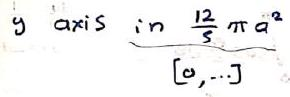
\includegraphics[max width=\textwidth]{2024_07_21_a4d038e3d75ef384087fg-3}
\end{center}

A $x=0 \mapsto \theta=\pi / 2, \quad \theta \in[0, \pi / 2]$

$$
\therefore s=2 \cdot \int_{0}^{\pi / 2} 2 \pi \cdot x d s \quad d s=\sqrt{\left(\frac{d x}{d \theta}\right)^{2}+\left(\frac{d y}{d \theta}\right)^{2}} d \theta
$$

$$
=4 \pi \times 3 a_{0}^{2} \int_{0}^{\pi / 2} \cos (\theta) \sin (\theta) d \theta
$$

$$
=3 a \sin (\theta) \cos (\theta) d \theta
$$

$$
=a \cdot 12 \pi a^{2} \cdot \frac{1}{5}=\frac{12 \pi a^{2}}{5}
$$

3 find length of carve $x=t^{2}, y=t^{3}$ t $\left.t 0,1\right]$

A. $\frac{d x}{d t}=2 t, \quad \frac{d y}{d t}=3 t^{2}$

$$
\therefore L=\int_{6}^{1} \sqrt{\left(\frac{d x}{d t}\right)^{2}+\left(\frac{d y}{d t}\right)^{2}} d t=\int_{0}^{2} \sqrt{\left(4 t^{2}+9 t^{4}\right)} d t
$$

$=\int_{0}^{1} t \sqrt{4+a t^{2}} d t$, let $4+9 t^{2}=u \Rightarrow \frac{d u}{d t}=18 t, d t=18 d \cdot d y$

$\equiv \int_{4}^{13} \sqrt{u} \frac{d u}{18}$

$t=[0,1] \Rightarrow u=[4,13]$

$$
=\frac{1}{27}\left[u^{3 / 2}\right]_{4}^{1 / 3}=\frac{1}{27}\left(13^{3 / 2}-4^{3 / 2}\right)
$$

\begin{enumerate}
  \setcounter{enumi}{3}
  \item Find the perimeter of cardioid $r=a(1+\cos (\theta))$
\end{enumerate}

A) Sine eqn remaims unchanged when $\theta=-\theta$ $\theta \in[0, \pi]$ $L=2 \iint_{0}^{\pi} \sqrt{r^{2}+\left(\frac{d r}{d \theta}\right)^{2}} d \theta, \quad \frac{d r}{d \theta}=-a \sin (\theta)$

$=2 \int_{0}^{\pi} \sqrt{a^{2}\left(1+\cos (\theta)^{2}+a^{2} \sin ^{2}(\theta)\right.} d \theta$

$=2 \int_{0}^{\pi} \sqrt{2 a^{2}(1+\cos (\theta))} d \theta=4 a \int_{0}^{\pi} \cos \frac{\theta}{2} d \theta$

$=8 a\left[\sin \frac{\theta}{2}\right]_{0}^{\pi}=8 a$

$$
\begin{aligned}
& \text { Volume of Solid od } \\
& \text { obtalned by revolving } y=f(x) \text { aboul } x \text {-ax.s;[a,b] } \\
& v=\int_{a}^{b} \pi y^{2} d x
\end{aligned}
$$

\begin{enumerate}
  \item Prove that the volume of a right circular cone of height $h$ and base radius $r$ is $1 / 3 \pi r^{2} h$
\end{enumerate}

A $\quad V=\int_{0}^{h} \pi y^{2} d x$

$$
y=r / h x
$$

$\therefore v=\int_{0}^{h} \pi \frac{r^{2}}{h^{2}} x^{2} d x=\pi \frac{r^{2}}{h^{2}} \cdot \frac{1}{3}\left[x^{3}\right]_{0}^{h}=\frac{1}{3} \pi r^{2} h$

\begin{enumerate}
  \setcounter{enumi}{1}
  \item Find the volume formed by revolution of loop of carve $y^{2}(a+x)=x^{2}(3 a-x)$ about $x$-axis
\end{enumerate}

le! $y=0 \Rightarrow x^{2}(3 a-x)=0 \Rightarrow x=0, x=3 a$

$$
\begin{aligned}
& \text { volume }=\int_{0}^{3 a} \pi y^{2} d x=\pi \int_{0}^{3 a} \frac{x^{2}(3 a-x)}{a+x} d x \\
& =\pi \int_{0}^{3 a} \frac{-x^{3}+3 a x^{2}}{a+x} \\
& =\pi \int_{0}^{3 a}\left(-x^{2}+4 a x-4 a^{2}+\frac{4 a^{3}}{x+a}\right) d x \\
& =\pi\left[-\frac{x^{3}}{3}+2 a x^{2}-\frac{4}{3} a^{3} x+4 a^{3} \ln (x+a)\right]_{0}^{3 a} \\
& =\pi\left[-9 a^{3}+18 a^{3}-12 a^{3}+4 a^{3} \ln (4 a)\right] \\
& =a^{3} \pi(-3+4 \ln (4)) \\
& \begin{array}{c}
\frac{-x^{2}+4 a x-4 a}{-x^{3}+3 a x^{2}} \\
\frac{-x^{3}-a x^{2}}{4 a x^{2}} \\
\frac{4 a x^{2}+4 a^{2} x}{-4 a^{2} x} \\
\frac{-4 a^{2} x-4 a^{3}}{4 a^{3}}
\end{array}
\end{aligned}
$$

\section*{Multiple integrals}
integrats undergoing

\section*{Double integrals}
\begin{enumerate}
  \item $\underbrace{2}_{0} \underbrace{2}_{\text {surdh. }} x_{0}^{x^{2}} x y \cdot d y \cdot d x$
\end{enumerate}

A limits of $y$ are $0 \rightarrow x^{2}$, limits of $x: 0 \rightarrow 2$

$$
\therefore \text { Ans: } \int_{0}^{2} x_{5}^{2} d x=\left[\frac{1}{2} \cdot \frac{x^{6}}{6}\right]_{0}^{2}=16 / 3
$$

\begin{enumerate}
  \setcounter{enumi}{1}
  \item $\int_{0}^{6} \int_{0}^{y^{3}} x^{2} y \cdot d y \cdot d x \Rightarrow \int_{0}^{5} \int_{0}^{y^{3}} x^{2} y \cdot d x \cdot d y$
\end{enumerate}

$$
=\int_{0}^{5}\left[y \cdot \frac{x^{3}}{3}\right]_{0}^{y^{3}} d y=\int_{0}^{5} y^{14} / 3 x d y=51 / 33
$$

\section*{Triple Integral}
\begin{enumerate}
  \item $\int_{0}^{1} \int_{0}^{2} \int_{0}^{2} x^{2} y z d x d y d z$
\end{enumerate}

$$
\begin{aligned}
& f y=y \\
& x y y
\end{aligned}
$$

A)

$\int_{0}^{1} \int_{0}^{2}\left(\int_{1}^{2} x^{2} \cdot y z \int_{1} d x\right) d y \cdot d x$.

$=\int_{0}^{1} \int_{0}^{2}\left[\frac{x^{2} y z^{2}}{2}\right]_{z^{1}}^{2} d y \cdot d x=\int_{0}^{1} \int_{0}^{2} \frac{x^{2} y \cdot 4-x^{2} y}{2} d y \cdot d x$

$=\int_{-0}^{1-2} \int_{0}^{2} \frac{3}{2} x^{2} y d y \cdot d x$

$$
\begin{aligned}
& =\int_{0}^{1}\left[\frac{3 x^{2} y^{2}}{4}\right]_{0}^{2} d x \\
& =\int_{0}^{1} 3 x^{2} d x=\left.x^{3}\right|_{0} ^{1}=1
\end{aligned}
$$

$2 \int_{-c}^{c} \int_{-b}^{b} \int_{-a}^{0}\left(x^{2}+y^{2}+z^{2}\right) d x d y \cdot d z$

A)

$$
\begin{aligned}
& \int_{-c}^{c} \int_{-b}^{b}\left(x^{2} z+y^{2} z+\frac{z^{3}}{3}\right)_{-a}^{a} d y \cdot d x-=\int_{-c}^{c} \int_{-b}^{b}\left(2 a x^{2}+2 a y^{2}+\frac{2}{3} a^{3}\right) d y \cdot d x \\
&=\int_{-1}^{c}\left[2 a x^{2} y+\frac{2 a y^{3}}{3}+\frac{2}{3} a^{3} y\right]_{-b}^{b} d x \\
&=\int_{-c}^{c}\left(4 a b x^{2}+\frac{4 a b^{3}}{3}+\frac{4}{3} a^{3} b\right) d x \\
& \Rightarrow\left[\frac{4 a b x^{3}}{3}+\frac{4}{3} a b^{3} x+\frac{4}{3} a^{3} b x\right]_{-c}^{c}=\frac{8}{3} a b c^{3}+\frac{8}{3} a b^{3} c+\frac{8}{3} a^{3} b c \\
&=\frac{8}{3} a b c\left(a^{2}+b^{2}+c^{2}\right)
\end{aligned}
$$

$3 \int_{-1}^{1} \int_{0}^{z} \int_{x-z}^{x+z}(x+y+z) d x d y d z$

$$
\begin{aligned}
& \frac{(x+z)^{2}}{2}-\frac{(x-z)^{2}}{2} \\
& =\frac{4 x z}{2}
\end{aligned}
$$

A) $\left.\rightarrow \int_{x-x}^{x+1}(x+y+z) d y\right]$

$$
I=\left[x y+\frac{y^{2}}{2}+z y\right]_{x-z}^{x+2}
$$

$$
\begin{aligned}
I= & x(x+z)+\frac{(x+z)^{2}}{2}+z(x+z) \\
& -\left(x(x-z)+\frac{(x-z)^{2}}{2}+z(x-z)\right) \\
= & x(2 z)+2 x z+z(2 z) \\
= & 2 x z+2 x z+2 x z^{2} \\
= & 4 x z+2 z^{2}
\end{aligned}
$$

$$
\begin{aligned}
& \int_{-1}^{1}\left[\int_{0}^{z}\left(4 x z+2 z^{2}\right) d x\right] d z \\
& \Rightarrow \int_{-1}^{1}\left(2 z^{3}+2 z^{3}\right) d z=\left[\frac{4 z^{4}}{4}\right]_{-1}^{1}=0
\end{aligned}
$$

\& $\int_{0}^{1} \int_{0}^{x} \int_{0}^{x+y}(2 x+y-z) d z d y d x$\\
A)

$$
\begin{aligned}
& I_{3}=\int_{0}^{x+2 y}(2 x+y-z) d z \\
& =\left[2 x z+y z-\frac{z^{2}}{2}\right]_{0}^{x+y}=2 x^{2}+2 x y+x y+y^{2}-\frac{(x+y)^{2}}{2} \\
& =2 x^{2}+3 x y+y^{2}-\frac{x^{2}+y^{2}+2 x y}{2} \\
& =\frac{3 x^{2}+y^{2}+4 x y}{2}
\end{aligned}
$$

\begin{center}
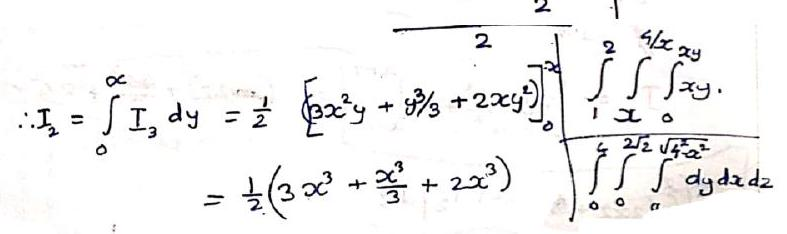
\includegraphics[max width=\textwidth]{2024_07_21_a4d038e3d75ef384087fg-4}
\end{center}

$$
\begin{aligned}
& \frac{1}{6}\left(9 x^{3}+6 x^{3}+x^{3}\right)=\frac{16 x^{3}}{6}=\frac{8}{3} x^{3} \\
& I=\int_{0}^{1} \frac{8}{3} x^{3} d x=\left[\frac{2}{3} x^{4}\right]_{0}^{1}=\frac{2}{3}
\end{aligned}
$$

\begin{enumerate}
  \setcounter{enumi}{4}
  \item $\int_{0}^{1} \int_{0}^{x} \int_{0}^{x+y}(2 x+y-1) d z d y d x$
\end{enumerate}

$$
\begin{aligned}
& \int_{0}^{1}\left(\int_{0}^{x}\left(2 x^{2}+2 x y+x y+y^{2}-x-y\right) d y\right) d x \\
= & \int_{0}^{1} \int_{0}^{x}\left(2 x^{2}+3 x y+y^{2}-x-y\right) d y d x \\
= & \int_{0}^{1}\left[2 x^{2} y+3 / 2 x y^{2}+y^{3} / 3-x y-y^{2} / 2\right]^{x} d x \\
= & \int_{0}^{1}\left(2 x^{3}+\frac{3}{2} x^{3}+\frac{x^{3}}{3}-x^{2}-\frac{x^{2}}{2}\right) d x \\
= & {\left[\frac{x^{4}}{2}+\frac{3 x^{4}}{8}+\frac{x^{4}}{12}-\frac{x^{3}}{3}-\frac{x^{3}}{6}\right]_{0}^{1}=\frac{1}{2}+\frac{3}{8}+\frac{1}{12}-\frac{1}{3}-\frac{1}{6} } \\
= & 11 / 24
\end{aligned}
$$

A $\int_{0}^{1} \int_{0}^{x}[2 x z+y z-z]_{0}^{x+y} d y d x$


\begin{align*}
& 6 \int_{1}^{2} \int_{x}^{4 / x} \int_{0}^{x y} x y \cdot d x d x d y \\
& \int_{1}^{2} \int_{x}^{4 / x}[x y z]_{0}^{x y} d x d y=\int_{1}^{2} \int_{x}^{6 / x} x^{2} y^{2} d y \cdot d x \\
&= \int_{1}^{2}\left[\frac{x^{2} y^{3}}{3}\right]_{x}^{4 / x} d x \\
&=\int_{1}^{2} \frac{x^{2}}{3}\left(\frac{64}{x^{3}}-x^{3}\right) d x=-4 \\
&=\int_{1}^{2}\left[\frac{64}{3} \cdot \frac{1}{x}-\frac{x^{5}}{3}\right] d x \\
&=\left[\frac{64}{3} \ln (x)-\frac{x^{6}}{18}\right]_{1}^{2}=\frac{64}{3} \ln (2)-\frac{64}{18}-\frac{64}{3} \ln (1)+\frac{1}{18} \\
&=\frac{64}{3} \ln (2)-\frac{63}{18}=\frac{64}{3} \ln (2)-\frac{7}{2}
\end{align*}


\begin{enumerate}
  \setcounter{enumi}{6}
  \item $\int_{0}^{4} \int_{0}^{2 \sqrt{2}} \int_{0}^{\sqrt{4 x-x^{2}}} d y \cdot d x d y$
\end{enumerate}

$$
\begin{aligned}
& =\int_{0}^{4} \int_{0}^{2 \sqrt{2}} \sqrt{4 z-x^{2}} d y \cdot d x d x= \\
& =\int_{0}^{4} \int \sqrt{2 \sqrt{2}} \sqrt{(2 \sqrt{z})^{2}-x^{2}} d x \cdot d z \\
& =\int_{0}^{4}\left[\frac{x}{2} \sqrt{4 z-x^{2}}+2 z \sin ^{-1}\left(\frac{x}{2 \sqrt{2}}\right)\right]_{0}^{2 \sqrt{2}} d z \\
& =\int_{0}^{4}(\sqrt{2} \sqrt{4 z-8}+\pi z) d x \\
& =\int_{0}^{4}(2 \sqrt{2} \sqrt{z-2}+\pi z) d z= \\
& =\left[2 \sqrt{2} \cdot \frac{2}{3}(z-2)^{3 / 2}+\frac{\pi z^{2}}{2}\right]_{0}^{4}=\frac{4}{3} \sqrt{2} 2^{3 / 2}+8 \pi-\frac{4 \sqrt{2}}{2}(-2)^{3 / 2}
\end{aligned}
$$

\begin{enumerate}
  \setcounter{enumi}{7}
  \item Calculate.
\end{enumerate}

$\iint r^{3} d r d \theta$ ever the area included between

circles $\gamma_{T}=2 \sin (\theta), \gamma_{2}=4 \sin (\theta)$\\
A) $r_{1}=2 \sin (\theta) \rightarrow \theta \in[0, \pi]$

$\therefore \int_{0}^{\pi} \int_{r=2 \sin (t)}^{r=4 \sin (\omega)} r^{3} d r . d \theta$

$$
\begin{aligned}
=\int_{0}^{\pi}\left[\frac{r^{4}}{4}\right]_{2 \sin (\omega)}^{4 \sin (\theta)} d \theta & =\int_{0}^{\pi}\left(\frac{4^{4}}{4} \cdot \sin ^{4}(\theta)-\frac{2^{4}}{4} \sin ^{4}(\theta)\right) d \theta \\
: & =\int_{0}^{\pi} 60 \sin ^{4}(\theta) d \theta=2 \cdot 6 \int_{0}^{\pi / 2} \sin ^{4}(\theta) d \theta \\
= & 2.60 \cdot\left[\frac{4-1)(4-3)}{4(4-2)}\right] \frac{\pi}{2}=120 \cdot \frac{3 \pi}{4}=\frac{45}{2} \pi
\end{aligned}
$$

$\begin{aligned}=\int_{0}^{\pi}\left[\frac{\gamma^{4}}{4}\right]_{2 \sin (\theta)}^{4 \cos (\theta)}=d \theta & =\int_{0}^{\pi}\left(64 \cdot \cos ^{4}(\theta)-4 \sin ^{4}(\theta)\right) d \theta \\ & =\int_{0}^{\pi}\left[64 \cos ^{4}(\theta)-4 \cdot\left(1-\cos ^{2}(\theta)\right)^{2}\right] d \theta\end{aligned}$

\begin{center}
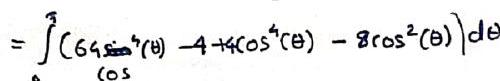
\includegraphics[max width=\textwidth]{2024_07_21_a4d038e3d75ef384087fg-5(1)}
\end{center}

$=\int_{0}^{4}\left(68 \cos ^{4}(\theta)-8 \cos ^{2}(\theta)-4\right) d \theta$

\section*{Change of order}
Here we find new limits by comparing actual limits $w \%$ using sketch.

\begin{itemize}
  \item Change the ordor of integration:
\end{itemize}

$$
\int_{0}^{1} \int_{0}^{x} f(x, y) d y \cdot d x
$$

\begin{enumerate}
  \setcounter{enumi}{3}
  \item Here limits of $y \geq\{[a \rightarrow$ is variable limit: $0 \leq y \leq x$
\end{enumerate}

limit of $x$ is constant: $0 \leq x \leq 1$

By changing the order if integration. limits of $x$ become variable \& that of $y$ becomes constant

$\therefore$ limits of $x=y \leq x \leq 1$

$y: 0 \leq y \leq 1<$

$\therefore$ cultered int:

$$
\int_{0}^{1} \int_{y}^{1} f(x, y) d x \cdot d y
$$

2.) Change order and eval:

$$
\int_{0}^{1} \int_{0}^{\sqrt{1-x^{2}}} y^{2} d y \cdot d x:=I
$$

A)

$$
\begin{aligned}
& y \in\left[0, \sqrt{1-x^{2}}\right], x \in[0,1] \\
& \text { or } 0 \leq y \leq \sqrt{1-x^{2}}, \\
& 0 \leq x \leq 1 \\
& \left.\sqrt{1-x^{2}}\right|_{0 \rightarrow 1} \Rightarrow[\sqrt{1}, 0] \\
& \therefore 0 \leq y \leq[1,0] \rightarrow 0 \leq y \leq 1 \\
& \left.y=\sqrt{1-x^{2}} \Rightarrow x=\sqrt{1-y^{2}}\right\}[1,0]
\end{aligned}
$$

\section*{$0 \leq x \leq \sqrt{1-y^{2}}$}
$I \equiv \int_{0}^{1} \int_{0}^{\sqrt{1-y^{2}}} y^{2} \cdot d x \cdot d y$

$=\int_{0}^{1} y^{2} \cdot \sqrt{1-y^{2}} d y$.

clet $y=\sin (u), \therefore d y=\cos (u) d u, u=\sin ^{-1}(y), \therefore[0,1] \mapsto[0, \pi / 2]$

$\therefore I=\int^{\pi / 2} \sin ^{2}(u) \sqrt{1-\sin ^{2}(u)} \cos (u) d u$

$0 \pi / 2$

\begin{center}
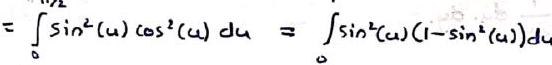
\includegraphics[max width=\textwidth]{2024_07_21_a4d038e3d75ef384087fg-5(3)}
\end{center}

$=\int_{0}^{\pi / 2} \sin ^{2}(u) d u-\int^{\pi / 2} \sin ^{4}(u) d u$

$=\frac{1}{2} \times \pi / 2 \rightarrow-\frac{3 \times 1}{4 \times 2} \times \frac{\pi}{2}=\pi / 16$\\
3. $\int_{0}^{4 a} \int_{x^{2} / 4 a}^{2 \sqrt{a x}} d y d x=I$

\begin{center}
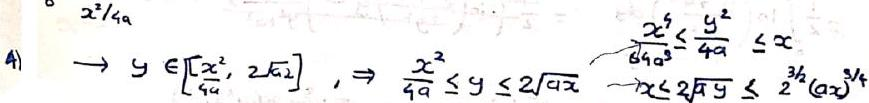
\includegraphics[max width=\textwidth]{2024_07_21_a4d038e3d75ef384087fg-5}
\end{center}

\begin{center}
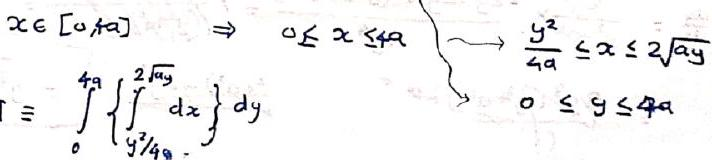
\includegraphics[max width=\textwidth]{2024_07_21_a4d038e3d75ef384087fg-5(2)}
\end{center}

$=\int_{0}^{4 a}\left(2 \sqrt{a y}-\frac{y^{2}}{4 a}\right) d y=\int_{0}^{4 a} 2 \sqrt{a} \sqrt{x y} d y-\int_{0}^{4 a} \frac{y^{2}}{4 a} d y$

$=2 \sqrt{a}\left[\frac{2 y^{3 / 2}}{3}\right]_{0}^{4 a}-\left[\frac{y^{3}}{12 a}\right]_{0}^{4 a}=\frac{4}{3} \sqrt{a} 4^{5 / 2} \cdot a^{5 / 2}-\frac{64 a^{3}}{12 a}$

$=\frac{32}{3} a^{2}-\frac{16}{3} a^{2}=\frac{16}{3} a^{2}$

$4 \int_{0}^{a} \int_{y}^{a} \frac{x}{x^{2}+y^{2}} d x \cdot d y$

$\rightarrow \quad 0 \leq 0 \leq \leq a$.

$y \leq x \leq a$

$I=\int_{0}^{a} \int_{y}^{a} \frac{x}{x^{2}+y^{2}} d x \cdot d y \quad$ let $u=x^{2}+y^{2}, \therefore \frac{d y}{d x}=2 x, d x=\frac{d u}{2 x}$

$=\int^{a} \int^{y^{2}+a^{2}} \frac{1}{2 a} d y . d y . \quad \therefore x \rightarrow[y, a] \longmapsto \underbrace{\left[2 y^{2}, y^{2}+a^{2}\right]}_{u-\text { spaue }}$

$=\int_{0}^{a}\left[\frac{1}{2} \ln (u)\right]_{2 y^{2}}^{y^{2}+a^{2}} d x y=\int_{0}^{a} \frac{1}{2} \ln \left(\frac{y^{2}+a^{2}}{2 y^{2}}\right) d y \leftarrow$ by parts

$=\frac{1}{2} \int_{0}^{9} \ln \left(\frac{y^{2}+a^{2}}{2 y^{2}}\right) d y$

$\frac{d_{4}}{d y}=\frac{2 y^{2}}{y^{2}+a^{2}} \times \frac{-2 y^{2} \cdot 2 y-\left(y^{2}+a^{2}\right) 4 y}{4 y^{4}}=\frac{-2 a^{2}}{y^{3}+a^{2} y}$

$\therefore I=\frac{1}{2}\left\{\ln \left(\frac{y^{2}+a^{2}}{2 y^{2}}\right) y-\int \frac{-2 a^{2} y}{y^{3}+a^{2} y} d y\right]_{0}^{a} d y$

for integral: $\int \frac{-2 a^{2} y}{y^{3}+a^{2} y}=\int \frac{-2 a^{2}}{y^{2}+a^{2}}=-2 a^{2} \int \frac{1}{y^{2}+a^{2}}$

$=-\frac{2 a^{2}}{a^{2}} \int \frac{1}{(y / a)^{2}+1} d y$

let $u=y / a . \therefore d y=d u \cdot a$

$$
\begin{aligned}
\rightarrow & =-2 a \int \frac{d y}{u^{2}+1}=-92 \tan ^{-1}(u)=-2 \tan ^{-1}\left(\frac{y}{a}\right) \\
& =\frac{1}{2}\left[\ln \left(\frac{y^{2}+a^{2}}{2 y^{2}}\right) \cdot y+2 a \tan ^{-1}\left(\frac{y}{a}\right)\right]_{0}^{9} \\
& =\frac{1}{2} \ln (-1) \cdot a+d \cdot \tan ^{-1}(1) \\
& =a \cdot \frac{\pi}{4}
\end{aligned}
$$


\end{document}